\documentclass{beamer}
%Imports and customization
\usepackage{tikz}
\usepackage{graphicx}
\usepackage{tikz-feynman}
\graphicspath{ 
    {./images/}
}

\beamertemplatenavigationsymbolsempty
\setbeamertemplate{sidebar right}{}
\setbeamertemplate{footline}{
    \hfill\usebeamertemplate***{navigation symbols}
    \hspace{1cm}\insertframenumber{}/\inserttotalframenumber
}
\setbeamertemplate{caption}{\raggedright\insertcaption\par}
\setbeamersize{text margin left=5mm,text margin right=5mm} 

\setbeamerfont{itemize/enumerate body}{size=\scriptsize}
\setbeamerfont{itemize/enumerate subbody}{size=\scriptsize}
\setbeamerfont{itemize/enumerate subsubbody}{size=\scriptsize}


%Custom Macros
\newcommand{\statwarn}{
    \tiny \color{red} Absolute numbers here mean NOTHING. Plots are based on small (100k events) samples, and are highly biased. All that matters is relative position!
}


\newcommand{\fullscreenimage}[2]{
    \frame{
        \frametitle{#1} 
        \begin{figure}
        \includegraphics[height=0.9\textheight,keepaspectratio]{#2}
        \end{figure}
    }
}


\newcommand{\displayone}[3]{
    \frame{
        \frametitle{#1} 
        \begin{columns}
            \begin{column}{0.5\textwidth}
                #2
            \end{column}
            \begin{column}{0.5\textwidth}
                \begin{figure}
                    \includegraphics[width=\linewidth,height=\textheight,keepaspectratio]{#3}
                \end{figure}
            \end{column}
        \end{columns}
    }
}

\newcommand{\displayonelarge}[3]{
    \frame{
        \frametitle{#1} 
        \begin{columns}
            \begin{column}{0.3\textwidth}
                #2
            \end{column}
            \begin{column}{0.7\textwidth}
                \begin{figure}
                    \includegraphics[width=\linewidth,height=\textheight,keepaspectratio]{#3}
                \end{figure}
            \end{column}
        \end{columns}
    }
}


\newcommand{\displaytwo}[4]{
    \frame{
        \frametitle{#1} 
        #2
        \begin{columns}
            \begin{column}{0.5\textwidth}
                \begin{figure}
                    \includegraphics[width=\linewidth,height=\textheight,keepaspectratio]{#3}
                \end{figure}
            \end{column}
            \begin{column}{0.5\textwidth}
                \begin{figure}
                    \includegraphics[width=\linewidth,height=\textheight,keepaspectratio]{#4}
                \end{figure}
            \end{column}
        \end{columns}
    }
}


\newcommand{\displaythree}[5]{
    \frame{
        \begin{columns}[T]
            \begin{column}{0.5\textwidth}
                \insertframetitle{#1}\\
                #2
            \end{column}
            \begin{column}{0.5\textwidth}
                \begin{figure}
                    \includegraphics[width=\linewidth,height=\textheight,keepaspectratio]{#3}
                \end{figure}
            \end{column}
        \end{columns}
        \begin{columns}[T]
            \begin{column}{0.5\textwidth}
                \begin{figure}
                    \includegraphics[width=\linewidth,height=\textheight,keepaspectratio]{#4}
                \end{figure}
            \end{column}
            \begin{column}{0.5\textwidth}
                \begin{figure}
                    \includegraphics[width=\linewidth,height=\textheight,keepaspectratio]{#5}
                \end{figure}
            \end{column}
        \end{columns}
    }
}


\newcommand{\announcesection}[1]{
    \section{#1}
    \frame{
        \begin{center}
            {\huge #1} 
        \end{center}
    }
}


%Begin Presentation
\begin{document}
    \title{Status Report on VBF/ggF Separation BDT}
    \author{Chris Milke}
    \institute{Southern Methodist University}
    \date{28 May, 2020}

    \frame{\titlepage}
    %{
    %    \usebackgroundtemplate{\includegraphics[width=\paperwidth]{dallashall_atlas}}
    %    \begin{frame} \titlepage \end{frame}
    %}
    %\frame{\frametitle{Overview} \tableofcontents}

    \section{Analysis Baseline Status}

\displayonelarge{VBF Selection Process Overview}{
    Selection of VBF events from data is done through a series of selection "filters"
}{cutflows/general}

\displayonelarge{VBF-Specific Selections}{
    {\tiny \begin{itemize}
        \item VBF Pair: Remove events in which there are fewer than two jets that are {\bf not} btagged
        \item VBF dEta: Select the jet pair with the highest invariant mass as the  "VBF Pair".\\Remove events where the $\Delta \eta$ of this pair is less than 3
        \item VBF mjj: Remove events where the "VBF Pair's" invariant mass is less than 1000 GeV
    \end{itemize} }
}{cutflows/vbf_only}

\displaytwo{ggF vs VBF for Various \cvv Values}{
    Current selection process across ggF and varying values of \cvv
}{cutflows/c2v_compare}{cutflows/c2v_compare_log}

    \fullscreenimage{Comparing Selection Performance}{roc_explanation}
\fullscreenimage{Current Selection Method Performance}{rocs/rocs_initial}

\displayonelarge{Baseline BDT}{
    As a baseline, train BDT with same inputs as current algorithm. It should perform at least as well.
}{rocs/rocs_bdt1}

\fullscreenimage{Adding Fox-Wolfram Moments to BDT}{fwMoment_ordering}
\displayfour{Fox-Wolfram Distributions}
{fw_moments/fox-wolfram_1}
{fw_moments/fox-wolfram_2}
{fw_moments/fox-wolfram_3}
{fw_moments/fox-wolfram_4}


\displaytwo{BDT with Fox-Wolfram Moments}{
    Improvent from first seven FW Moments is minor, but noticeable.
}{rocs/rocs_bdt2}{rocs/rocs_bdt2_zoom}


\frame{
    \frametitle{Exploring Multi-Jet Discriminants: Centrality}
    \begin{columns}
        \begin{column}{0.5\textwidth}
            {\small The VBF initial scatter quark jets are not always the only thing present in VBF events.
            Radiated Jets (ISR \& FSR) are not uncommon, and provide additional handles for analysis.}
            \begin{figure}
                \includegraphics[width=\linewidth,height=\textheight,keepaspectratio]{ event_display}
            \end{figure}
        \end{column}
        \begin{column}{0.5\textwidth}
            \begin{center}\resizebox{0.40\textheight}{!}{ 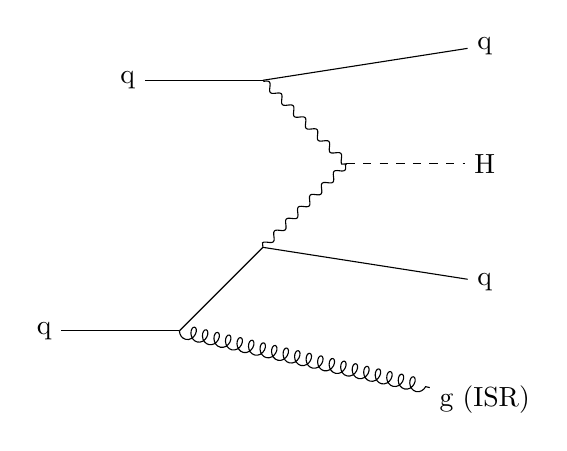
\begin{tikzpicture} \begin{feynman}
    \vertex (a);
    \vertex [right=of a] (b) {H};
    \vertex [above left=of a] (vb1);
    \vertex [below left=of a] (vb2);
    \vertex [left=of vb1] (q1i) {q};
    \vertex [below left=of vb2] (q2k);
    \vertex [left=of q2k] (q2i) {q};
    \vertex [above =of b] (q1f) {q};
    \vertex [below =of b] (q2f) {q};
    \vertex [below =of q2f] (g) {g (ISR)};

    \diagram* {
        (q1i) -- (vb1) -- (q1f),
        (q2i) -- (q2k) -- (vb2) -- (q2f),
        (q2k) --[gluon] (g),
        (vb1) -- [boson] (a) -- [boson] (vb2),
        (a) -- [scalar] (b),
    };
\end{feynman} \end{tikzpicture}
 }\end{center}
            \begin{center}\resizebox{0.40\textheight}{!}{ \begin{tikzpicture} \begin{feynman}
    \vertex (a);
    \vertex [right=of a] (b) {H};
    \vertex [above left=of a] (vb1);
    \vertex [below left=of a] (vb2);
    \vertex [left=of vb1] (q1i) {q};
    \vertex [left=of vb2] (q2i) {q};
    \vertex [below right=of vb2] (q2k);
    \vertex [above =of b] (q1f) {q};
    \vertex [below =of b] (q2f) {q};
    \vertex [below =of q2f] (g) {g (FSR)};

    \diagram* {
        (q1i) -- (vb1) -- (q1f),
        (q2i) -- (vb2) -- (q2k) -- (q2f), 
        (q2k) --[gluon] (g),
        (vb1) -- [boson] (a) -- [boson] (vb2),
        (a) -- [scalar] (b),
    };
\end{feynman} \end{tikzpicture}
 }\end{center}
        \end{column}
    \end{columns}
}


\fullscreenimage{Centrality Distribution}{centrality}
\displaytwo{Centrality as a BDT Input}{
    Improvement from Centrality is very small,
    but there may be more to be gained with further study.
}{rocs/rocs_centrality}{rocs/rocs_centrality_zoom0}


    \section{Conclusion}
    \frame{
        \frametitle{Conclusions}
        \begin{itemize} {
            {\large \item Initial attempt at BDT with Fox-Wolfram moments is an improvement, but only barely}
            {\large \item Current Fox-Wolfram moments may be bugged, investigation ongoing}
            {\large \item More inputs and integration into main framework is coming soon!}
        } \end{itemize}
    }

    \announcesection{Backup}
    \fullscreenimage{BDT Input Ranking}{feature-importance_mjj_deta_FW_3}
    \fullscreenimage{BDT Overtraining Check}{ot-check_mjj_deta_FW_3}
    \input{fox_wolfram_dump.tex}
\end{document}
